\chapter{Experiments And Results}
\label{ch:results}

This chapter reports what the method of \autoref{ch:method} does when it is run. It has two parts, which follow the two levels of the pipeline. \autoref{sec:inner-loop-experiments} isolates the inner loop: the outer loop is switched off, the bodies are given rather than selected, and the question is what the evolved rules add to a base controller on a body that does not change, first to the generalist, on bodies it has never flown, then to a specialist, on the one body it was trained for. \autoref{sec:codesign-experiments} runs the whole pipeline and compares it with the morphology-only control of \autoref{subsec:pipeline-control} on the terms set by \autoref{ch:challenges}: whether an adaptation as cheap as this one changes which bodies the search finds.

Every experiment of the chapter uses the controllers, the plastic layer, the courses and the flights of \autoref{ch:method}, with the values of \autoref{tab:hebbian-parameters}, \autoref{tab:evaluation-courses} and \autoref{tab:pipeline-settings}; where an experiment departs from them, the departure is stated with the result it belongs to. The base controllers are the generalist of \autoref{subsec:generalist-training}, trained once, and the specialists of \autoref{subsec:specialist-training}, of which three were trained for the reference drone with the same settings and different random seeds; unless a specialist is numbered, the first of them is meant. The evolutionary algorithms are taken from their reference implementations, CMA-ES from pycma 4.4.4 \cite{hansen2019pycma} and NSGA-II from DEAP 1.4.3 \cite{fortin2012deap}; the networks run in PyTorch 2.10 \cite{paszke2019pytorch} and the simulation in Genesis 0.3.7 \cite{genesis2024}. A run is identified by its random seed, which fixes the samples of CMA-ES, the forests and, where there is one, the first population of bodies. \autoref{tab:results-runs} lists the runs of the chapter.
% PROVENANCE: library versions from reproducibility/environment.txt of the runs (cma==4.4.4, deap==1.4.3, torch==2.10.0);
% Genesis 0.3.7 = the vendored genesis/ (chapter 4). Specialists: wp1_bix_single_65536_lstm_15_r0..r2; "the first" = r1
% (the one used in the generalist-vs-specialist run and in the first rules-on-specialist run), second = r0, third = r2.

\begin{table}[htbp]
\centering
\begin{tabularx}{\textwidth}{>{\raggedright\arraybackslash}p{1.6cm} >{\raggedright\arraybackslash}p{2.0cm} >{\raggedright\arraybackslash}p{2.6cm} >{\raggedright\arraybackslash}p{2.0cm} >{\raggedright\arraybackslash}X >{\raggedright\arraybackslash}p{1.6cm}}
\hline
Section & Base controller & Bodies & Flights per generation & Measured at every generation, on new forests & Runs, generations \\
\hline
\ref{subsec:results-generalist} & generalist & 64 drawn at random, moved every 4 generations & 245\,760 & the best rules and the frozen generalist on the reference drone, 4\,096 forests & 1, of 50 \\
\ref{subsec:results-generalist} & generalist & the reference drone & 12\,800 & the best rules, the frozen generalist and a frozen specialist, 2\,048 forests & 2, of 200 \\
\ref{subsec:results-specialist} & a specialist & the reference drone & 12\,800 & the best rules, the frozen specialist and the frozen generalist, 2\,048 forests & 3, of 200, one per specialist \\
\hline
\end{tabularx}
\caption[Runs of this chapter]{Runs of this chapter. Every run uses 64 sets of rules per generation, the search course and the noise of \autoref{subsec:evaluation-flights}; a flight of the search is one set of rules, one body and one forest.}
\label{tab:results-runs}
\end{table}
% Rows checked 2026-09-25 against the finished local runs (src/WP2/experiments/thesis_inner_loop/): generalist seeds 5535 and 5536,
% specialists r1/r0/r2 with seeds 5535/5536/5537, all 200 generations, all exit 0.
% TODO: rows for section 6.2 (8 co-design runs: 4 of 2026-08-10 + 4 of batch_5, and 8 paired morphology-only runs with
%   the same seeds; see THESIS_DECISIONS.md section 6) when that section is written.

\section{Inner Loop Experiments}
\label{sec:inner-loop-experiments}

The inner loop of \autoref{subsec:inner-loop} was designed to run inside the outer loop, on bodies that the outer loop keeps replacing. Run on its own, on bodies that are given once and for all, it answers a narrower question, which is nevertheless the first that has to be asked: whether the rules add anything to a base controller at all, and what. On a fixed body nothing varies from one flight to the next but the forest, the commanded speed and the noise; the body, which \autoref{subsec:hebbian-why-output} presented as the quantity that varies between lifetimes and that fixed weights cannot anticipate, is the same in every flight. It is therefore the setting in which the argument for plasticity promises the least, and the one in which whatever the rules do can be read most clearly, because the frozen base controller flies the same body under the same conditions and any difference between the two is the work of the rules.

Two experiments are reported. In the first the base is the generalist, which flies every body as a compromise (\autoref{subsec:generalist-training}). The rules are evolved on many bodies, as in the pipeline, and then on the reference drone alone, and the specialist trained for that drone gives the scale of what the generalist leaves on the table there. In the second the base is a specialist, a controller that was trained for the body it flies and has nothing to recover; there are three of them, and the experiment is run on each.

\subsection{Recovering Performance on Generalist Controllers}
\label{subsec:results-generalist}

The first experiment runs the inner loop as the pipeline runs it, with one change: the bodies are not selected. Sixty-four bodies are drawn at random, as in the first generation of a run, with the reference drone excluded, and every four generations each gene of each body is moved by a Gaussian step of standard deviation 0.02 in the unit cube, so that the population keeps changing under the rules, as it does in a run, but drifts as a random walk instead of following the objectives. Fifty generations are run, with twelve such refreshes, and with the population, the flights and the fitness of \autoref{tab:pipeline-settings}: 64 sets of rules, 245\,760 flights of the search course per generation, forests drawn anew at every generation. At every generation the frozen generalist flies the same bodies on the same forests, and the best set of rules of the generation and the frozen generalist fly the reference drone on 4\,096 further forests of the search course that the search never sees, which is the measurement described in \autoref{subsec:pipeline-run}. The experiment thus shows the progress of the inner loop on the bodies it is given and on one it is not.
% PROVENANCE: logs/remote/wp2_evolution/wp2_mutation_4_bix_validation_lstm_15_r0/2026-06-13_02-23-30_mutation_4_bix_validation_lstm_15
% (IZAR, 27 h; catalog.mutate true, mutation_std 0.02, refresh_urdfs_every 4, include_standard_mydrone false, seed 67;
% production checkpoint, md5-identical to batch_5). Numbers: tesis/images/06_Results_and_Experiments/inner_loop/inner_loop_stats.json, "A".

\begin{figure}[htbp]
\centering
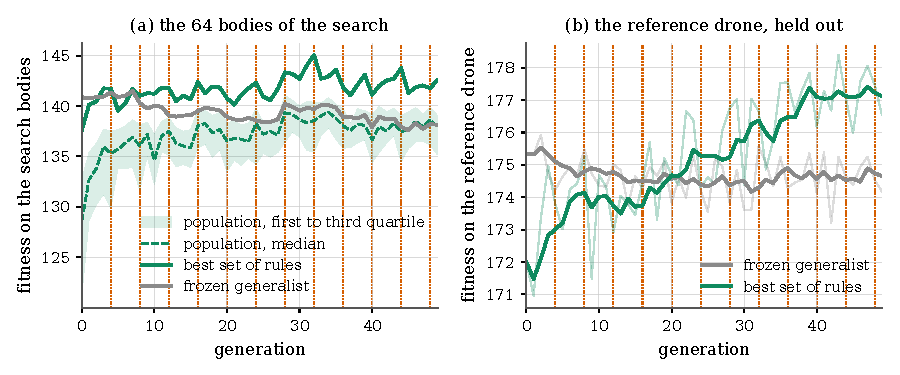
\includegraphics[width=\textwidth]{images/06_Results_and_Experiments/inner_loop/inner_loop_bodies.pdf}
\caption[The inner loop on 64 random bodies]{The inner loop on 64 random bodies. (a) Fitness on the bodies of the search: the best of the 64 sets of rules of each generation, the population's median with a band from the first to the third quartile, and the frozen generalist on the same bodies and forests. The dotted lines mark the refreshes of the bodies. (b) The best set of rules of each generation and the frozen generalist on the reference drone, which the search never flies, over 4\,096 new forests per generation; thin lines are the raw values, thick lines a moving average over five generations.}
\label{fig:inner-loop-bodies}
\end{figure}

\autoref{fig:inner-loop-bodies}(a) shows the fitness on the bodies of the search. At the first generation every one of the 64 sets of rules flies worse than the frozen generalist: the population's median is 129 against 141 for the frozen controller, and its best 138. This is the starting point that \autoref{subsec:inner-loop} chose: the rules begin as small perturbations of a controller that flies, and a perturbation, on average, costs. From there CMA-ES moves. From the seventh generation on the best set of rules of each generation is above the frozen controller, and over the last ten generations it exceeds it by 3.9, 142.2 against 138.2, a gain of about 3\,\%; the step size has shrunk from 0.074 to 0.058 in the meantime. The population's median, however, only catches up with the frozen controller, 137.9 against 138.2 over the same generations, and its upper quartile barely passes it: the search has found a direction in which the rules help, but a random perturbation around that direction still costs about as much as the direction gains, and the population as a whole never becomes clearly better than no rules at all. The curve of the frozen controller is not flat, because at every refresh the bodies change and the new population flies a little differently; this is the reason given in \autoref{subsec:pipeline-run} why the fitness of the rules cannot be compared across updates of the bodies, and the comparison that the figure allows is the one that holds at every generation, between the rules and the frozen controller on the same bodies and forests.

Panel (b) is the same comparison on a body that the search never flies. On the reference drone the best rules of the first generation are worse than the frozen generalist by 3.4, and they remain worse for the first four phases, sixteen generations: rules selected on other bodies do not transfer at once. From the sixth phase on the sign is reversed, and over the last ten generations the best rules exceed the frozen controller by $2.5 \pm 0.6$ on the reference drone, 177.1 against 174.6, or 1.4\,\%. The uncertainty is the spread over generations of the paired difference, each measured on 4\,096 fresh forests; the fitness of the frozen controller alone varies by 0.6 from one generation's forests to the next, so the gain is well above what a draw of forests can produce. It is also two thirds of what the rules gain on the bodies they are evolved on, which is the expected direction: part of what a set of rules gains is specific to the bodies on which it was selected.

\begin{figure}[htbp]
\centering
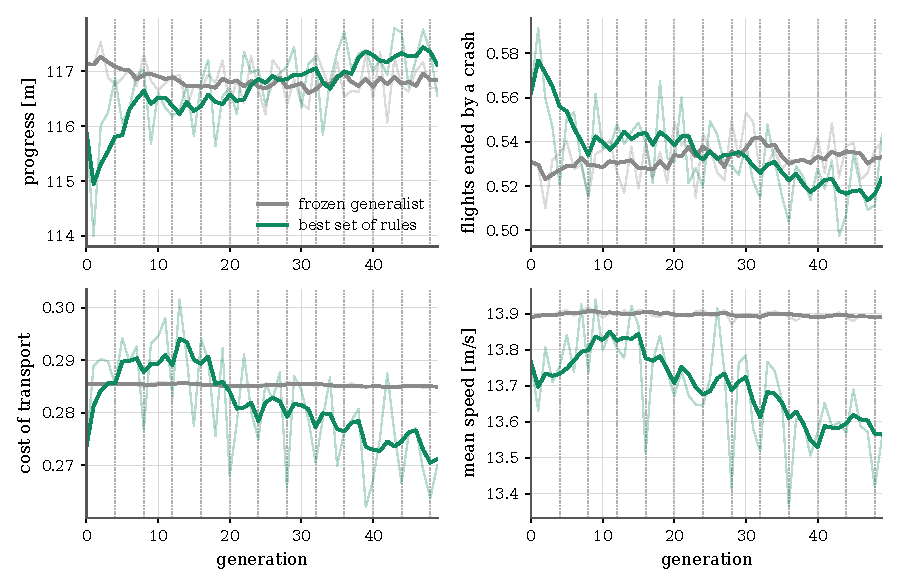
\includegraphics[width=\textwidth]{images/06_Results_and_Experiments/inner_loop/inner_loop_bodies_metrics.pdf}
\caption[Flights of the reference drone under the rules evolved on 64 bodies]{The flights of the reference drone in the experiment of \autoref{fig:inner-loop-bodies}, best set of rules against frozen generalist on the same 4\,096 forests per generation: progress, fraction of flights ended by a crash in the sense of \autoref{subsec:reward}, cost of transport and mean speed along the corridor. Thin lines are the raw values, thick lines a moving average over five generations.}
\label{fig:inner-loop-bodies-metrics}
\end{figure}

\autoref{fig:inner-loop-bodies-metrics} decomposes the held-out gain into the quantities of the flights. Progress and the fraction of flights that end in a crash barely move: 117.2~m against 116.8~m, and 52\,\% of the flights lost against 53\,\%, on a course that ends at five trees per metre. What moves is the speed, which the rules lower by 2\,\%, from 13.9 to 13.6~m/s over commands between 10 and 20~m/s, and the energy, which they lower more, by 4\,\% per metre. The rules do not make the generalist a better pilot of the reference drone in the sense in which a specialist is one; they make it fly the same course, with the same losses, a little slower and cheaper, and the reward pays for the change: its energy term rewards the saving directly, and its tracking term, a bell curve that is flat near the commanded speed, costs a flight a few per cent slower almost nothing per step while the flight lasts longer over the same distance. The first generations show the opposite, a cost of transport above that of the frozen controller, and the search passes through it: which term of the reward the rules end up serving is not decided at the start.

How much of what the generalist loses on the reference drone is this? The specialist trained for that drone gives the measure. In a second run the rules were evolved on the reference drone alone, with the same population and 200 forests for each set of rules, 12\,800 flights per generation, for 200 generations, and at every generation the best set of rules, the frozen generalist and the frozen specialist flew 2\,048 fresh forests of the search course. \autoref{fig:inner-loop-reference}(a) shows the three curves. The frozen generalist scores 174.5 on the reference drone and the specialist 182.2: a gap of 7.7, or 4\,\%, which is the price of the compromise of \autoref{sec:challenge-morphology} on a body of ordinary proportions. The rules, evolved on this body alone, recover $3.4 \pm 1.2$ of it over the last fifty generations, 44\,\% of the gap; the gain appears within the first twenty generations, reaches 3 by the sixtieth and hardly moves afterwards. The gap itself depends on which specialist is used as the measure: the three that were trained score 182.2, 189.7 and 182.4 on the same kind of forests (\autoref{subsec:results-specialist}), so that the rules recover between a quarter and a half of what a specialist has over the generalist.
% PROVENANCE: logs/runs_hebbian/2026-09-24_20-15-15_rules_on_generalist_s5535 (local, 200 gens, seed 5535, specialist r1;
% 22:15 → 03:17 on 2026-09-25, exit 0). Window = generations 150 to 199. inner_loop_stats.json, "G"[first entry].

\begin{figure}[htbp]
\centering
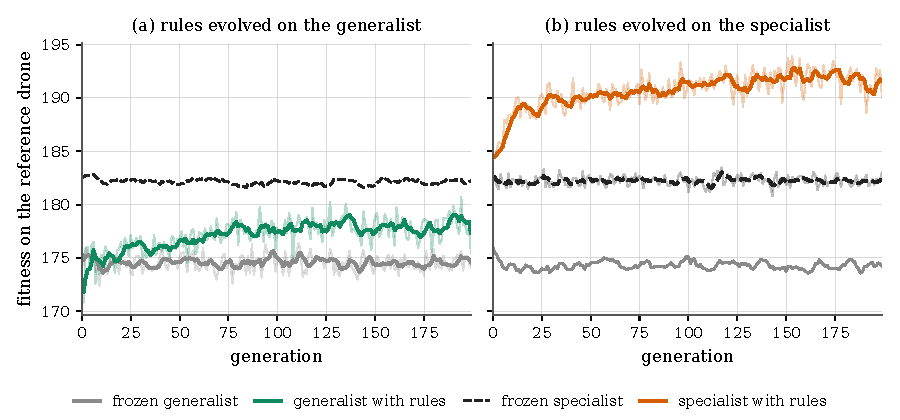
\includegraphics[width=\textwidth]{images/06_Results_and_Experiments/inner_loop/inner_loop_reference.pdf}
\caption[The inner loop on the reference drone alone]{The inner loop on the reference drone alone, fitness over 2\,048 new forests per generation, flown by every controller of a panel. (a) Rules evolved on top of the generalist, with the frozen generalist and the frozen specialist. (b) Rules evolved on top of the first specialist, with that specialist frozen and the frozen generalist. Thin lines are the raw values, thick lines a moving average over five generations.}
\label{fig:inner-loop-reference}
\end{figure}

\begin{figure}[htbp]
\centering
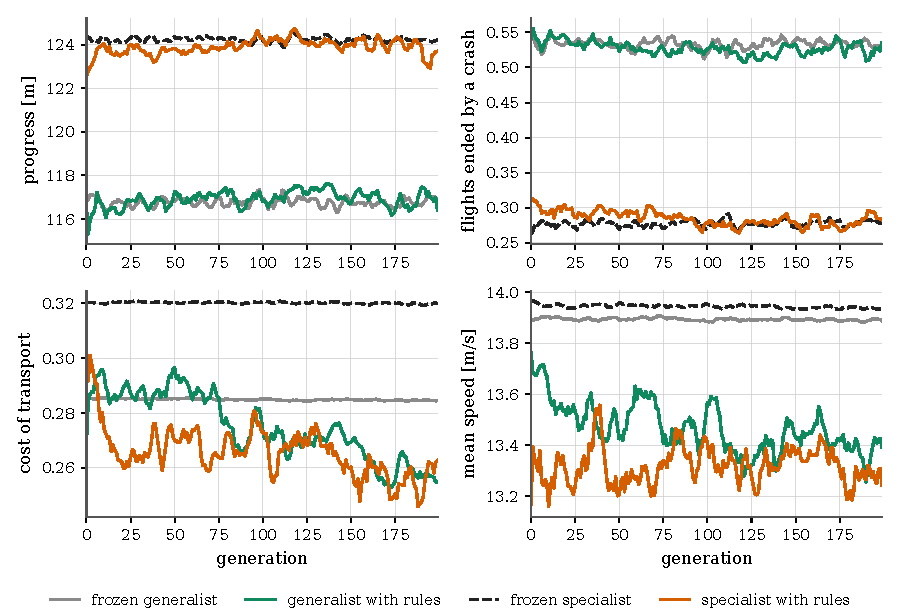
\includegraphics[width=\textwidth]{images/06_Results_and_Experiments/inner_loop/inner_loop_reference_metrics.pdf}
\caption[Flights of the reference drone under the four controllers]{The flights of the reference drone in the two runs of \autoref{fig:inner-loop-reference}: the generalist and the first specialist, frozen and with the best rules of each generation, on 2\,048 new forests per generation. Progress, fraction of flights ended by a crash, cost of transport and mean speed along the corridor; moving averages over five generations.}
\label{fig:inner-loop-reference-metrics}
\end{figure}

But the two gains are of a different kind, and \autoref{fig:inner-loop-reference-metrics} shows it. The specialist loses 28\,\% of its flights where the generalist loses 53\,\%, and covers 124~m where the generalist covers 117; it flies at much the same speed, 14.0 against 13.9~m/s, and it spends more per metre, with a cost of transport of 0.32 against 0.28. The rules leave the losses and the progress where the generalist has them and lower the cost of transport by 9\,\%, to 0.26, at a speed 3\,\% lower. Measured in reward, the rules recover over two fifths of the gap; measured in what the body does, they recover none of the specialist's advantage, which lies in avoiding the trees, and find instead an economy that the specialist never looked for. In the terms of the objectives of \autoref{subsec:outer-loop} the two changes are not on the same axis: the specialist moves the body along progress and pays for it in energy, the rules move it along the cost of transport at constant progress. This is the approximate correspondence between the reward and the objectives of which \autoref{subsec:reward} warned, seen from the side of the search: a change that the reward pays for need not be the change that a specialist would have made.

Two further observations from this run are used later. The fitness with which the best set of rules is selected, on the forests of the search, is 182.0 over the last fifty generations, against 177.9 for the same set of rules on the held-out forests: the maximum of 64 noisy measurements is optimistic by about 4, and a set of rules that is the best of its generation by that margin has often only been lucky on that generation's forests. This is one of the reasons why the pipeline judges the bodies on new forests and under eight sets of rules rather than one (\autoref{subsec:outer-loop}). And the run was repeated: twice with the same seed, for 100 and for 200 generations, and once with another seed for 200. Runs with the same seed diverge in the simulator, as every run does (\autoref{subsec:genesis-proscons}), and the three repeats agree with the first in the result, with gains of 3.0, 4.5 and $3.6 \pm 1.0$ over their last quarters and the same decomposition into speed and energy.
% PROVENANCE: winner's curse = search_best_last - val_best_last of the 200-gen run; repeats = run C
% logs/runs_hebbian/2026-07-08_09-59-42_validation_wspecialis_15_no_bix_15_lstm (100 gens, gain gens 75-99 +3.0) and run B
% logs/runs_hebbian/2026-06-10_10-40-16_validation_wspecialist_no_bix_15_lstm (200 gens, gain gens 150-199 +4.5; its
% "specialist" line is a 25-step specialist and is not used) and the second seed logs/runs_hebbian/2026-09-25_09-11-59_rules_on_generalist_s5536
% (200 gens, seed 5536, specialist r0 as third line: gain gens 150-199 +3.57 ± 0.97, CoT 0.261/0.285, speed 13.33/13.89).

\subsection{Improving Performance on Specialist Controllers}
\label{subsec:results-specialist}

The second experiment repeats the last one with a specialist in the place of the generalist, once for each of the three specialists trained for the reference drone. The rules are evolved on top of the frozen specialist, on the reference drone, with the same population, the same 12\,800 flights per generation and 200 generations, and at every generation the best set of rules, the frozen specialist and the frozen generalist fly 2\,048 fresh forests. \autoref{subsec:specialist-training} left the outcome open. A specialist was trained for the body it flies, and the argument of \autoref{subsec:hebbian-why-output}, that plasticity is selected when something varies between lifetimes, gives the rules nothing to work on here: the body is the one the weights were trained for. If what the rules do is adapt a controller to its body, this is where they should add the least.
% PROVENANCE: logs/runs_hebbian/2026-09-24_16-47-43_rules_on_specialist_r1_s5535 (first specialist), 2026-09-25_01-17-04_rules_on_specialist_r0_s5536
% (second), 2026-09-25_05-45-56_rules_on_specialist_r2_s5537 (third); local, seeds 5535/5536/5537, all exit 0; the "specialist_*" columns of their
% validation_summary.csv hold the frozen generalist. Window = generations 150 to 199. inner_loop_stats.json, "S". Generalist row of the table = run 2.

\begin{table}[htbp]
\centering
\small
\begin{tabularx}{\textwidth}{>{\raggedright\arraybackslash}X r r r r r r r r r}
\hline
 & \multicolumn{4}{c}{frozen} & \multicolumn{5}{c}{with the best rules} \\
Base controller & fitness & speed & CoT & crashes & fitness & gain & speed & CoT & crashes \\
\hline
generalist & 174.5 & 13.9 & 0.285 & 53\,\% & 177.9 & +3.4 & 13.4 & 0.259 & 53\,\% \\
first specialist & 182.2 & 13.9 & 0.320 & 28\,\% & 191.9 & +9.6 & 13.3 & 0.257 & 28\,\% \\
second specialist & 189.7 & 13.3 & 0.215 & 31\,\% & 190.2 & +0.5 & 13.3 & 0.212 & 34\,\% \\
third specialist & 182.4 & 13.9 & 0.344 & 29\,\% & 192.3 & +9.9 & 13.3 & 0.243 & 28\,\% \\
\hline
\end{tabularx}
\caption[The four base controllers on the reference drone, frozen and with the best rules]{The four base controllers on the reference drone, frozen and with the best set of rules of each generation, over the last fifty generations of their runs: fitness, mean speed along the corridor in m/s, cost of transport and fraction of flights ended by a crash, on 2\,048 new forests per generation. The gain is the difference in fitness between the two, measured on the same forests; its spread over generations is 1.2, 1.2, 1.0 and 0.8 from top to bottom.}
\label{tab:inner-loop-bases}
\end{table}

\autoref{tab:inner-loop-bases} gives the answer, and it is not the same for the three. On the first and the third specialist the rules add more than anywhere else in this section: $9.6 \pm 1.2$ and $9.9 \pm 0.8$, over 5\,\%, three times what they added to the generalist. \autoref{fig:inner-loop-reference}(b) shows the first: the rules are above the frozen specialist from the first generation, by 1.8 at generation 0 and by 4.3 over the first ten, the gain reaches 7.8 by the fortieth generation and 9.0 by the hundredth, and the third specialist follows the same course. On the second specialist the rules add nothing: $0.5 \pm 1.0$, negative over the first ten generations and inside the noise ever after.

The frozen controllers explain the difference. The three specialists were trained with the same settings and differ in the random seed alone, and they did not arrive at the same way of flying the reference drone. The first and the third fly it at 13.9~m/s with a cost of transport of 0.32 and 0.34, dearer than the generalist; the second flies it at 13.3~m/s with a cost of transport of 0.215, and scores 7.5 more than the other two for it, with the same progress and the same crashes. The rules bring the first and the third down to 13.3~m/s and to 0.26 and 0.24, with progress and crashes untouched, as they brought the generalist from 13.9 to 13.4~m/s and from 0.285 to 0.259; the second is there already, and they leave it where it is. Two further differences from the generalist's run are worth noting on the first specialist. The gain is there from the start, in the first generation, drawn with the same seed in the two runs, whereas on the generalist the best of the first generation was worse than no rules at all; and the selection is less deceived by its own forests, since the best fitness on the search forests exceeds the held-out fitness of the same rules by 2.5 instead of 4, the flights of a specialist varying less from one forest to the next, as its fewer crashes suggest.

Where the four bases end up is the remarkable part, and \autoref{fig:inner-loop-reference-metrics} shows it for the first two. Under their respective rules the generalist and the three specialists all fly the reference drone at the same speed, 13.3 to 13.4~m/s, three of them from 13.9; the cost of transport ends between 0.21 and 0.26, in the order in which the frozen controllers had it, and progress and crashes stay where each frozen controller had them. The rules do not move each controller by a fixed amount: they move each one towards a slower and cheaper flight of the same course, the flight that the fitness of \autoref{subsec:inner-loop} rewards on this body, and what each controller gains is the distance it had to travel to get there: nothing for the specialist that was there already, 3.4 for the generalist, about ten for the two specialists that flew fastest and dearest. Why the training reached this point with one seed and not with the other two, the experiment does not say; the training optimizes the discounted return of \eqref{eq:generalist-objective} from randomized releases and the search the reward summed over a flight from a fixed one, and the two are not the same measure of a flight.

\begin{table}[htbp]
\centering
\small
\begin{tabularx}{\textwidth}{>{\raggedright\arraybackslash}X r r r r r r r r}
\hline
 & \multicolumn{4}{c}{rules evolved on the generalist} & \multicolumn{4}{c}{rules evolved on the first specialist} \\
Controller & fitness & gain & crashes & CoT & fitness & gain & crashes & CoT \\
\hline
no rules & 174.6 &  & 53\,\% & 0.282 & 182.2 &  & 27\,\% & 0.318 \\
best set of rules & 178.3 & +3.7 & 51\,\% & 0.249 & 192.2 & +10.0 & 27\,\% & 0.253 \\
same, $D$ set to zero & 163.4 & $-11.2$ & 64\,\% & 0.267 & 185.1 & +2.9 & 38\,\% & 0.262 \\
same, $A$, $B$, $C$ set to zero & 174.2 & $-0.4$ & 55\,\% & 0.275 & 184.1 & +1.9 & 31\,\% & 0.286 \\
\hline
mean of the search & 179.0 & +4.4 & 51\,\% & 0.246 & 192.7 & +10.5 & 27\,\% & 0.259 \\
same, $D$ set to zero & 174.3 & $-0.3$ & 54\,\% & 0.265 & 186.3 & +4.1 & 30\,\% & 0.289 \\
same, $A$, $B$, $C$ set to zero & 178.5 & +3.9 & 51\,\% & 0.267 & 182.2 & +0.0 & 35\,\% & 0.281 \\
\hline
\end{tabularx}
\caption[The rules taken apart on the reference drone]{The rules taken apart on the reference drone. Each controller flies the same 2\,048 forests of the search course as the others in its column, four times with new forests; the table gives the mean fitness, its difference from the controller without rules, the fraction of flights ended by a crash and the cost of transport. The best set of rules is the one with the highest fitness in the run, the mean of the search is the centre of the CMA-ES distribution at the end of the run; $D$ set to zero leaves the terms that depend on the activity, $A$, $B$, $C$ set to zero leaves the constant term alone.}
\label{tab:d-ablation-fixed}
\end{table}

Is this retuning a constant shift of the output weights, which \autoref{subsec:hebbian-decay} showed that the term $D$ alone produces, or does it need the terms that respond to the activity? \autoref{tab:d-ablation-fixed} takes the rules of the generalist run and of the first specialist run apart. The best set of rules of each run, and the mean of its search, which is the centre of the distribution that CMA-ES arrived at rather than one lucky sample of it, fly the reference drone in three forms: as they are, with $D$ set to zero, and with $A$, $B$ and $C$ set to zero, all on the same forests. The gain does not split into a static part and a plastic part, and the two bases split it differently. On the generalist the centre of the search works almost entirely through $D$, which alone gives 3.9 of its 4.4 while the three other terms alone give nothing; on the best sample, however, the three terms alone are destructive, eleven points below no rules with two thirds of the flights lost, and $D$ is what makes them flyable. On the specialist $D$ alone gives nothing, or 1.9 on the best sample; $A$, $B$ and $C$ alone give a third of the gain and cost crashes, 38\,\% of the flights against 27; together the two give ten. In both cases the terms that depend on the activity make the drone crash more when they act alone, $D$ alone never does much harm, and the search has tuned the two against each other: the gain is a property of the pair. What the ablation excludes is the simplest reading, that the rules amount to a constant offset of the trained weights. On the specialist such an offset does nothing, and on the generalist it accounts for the centre of the search but not for the samples around it, which are what the pipeline flies.
% PROVENANCE: tesis/scripts/d_ablation_fixed_body.py → images/06_Results_and_Experiments/inner_loop/d_ablation_fixed_body.json
% (2026-09-24, local docker; 7 controllers × 2 048 forests × 4 repeats per run). Rows generated from the JSON.

This settles how the gains of this section are to be read. On the generalist the rules recover over two fifths of the gap to a specialist, in reward; but two specialists gain more from the same rules, and the third, which flies slow and cheap already, gains nothing, so the gain is not a recovery of what the generalist lacks on the reference drone. It is a retuning of the operating point of the flight, slower and cheaper at equal progress, that any base controller accepts when it has room for it and that the summed reward pays for, on a controller trained for the body as much as on one that was not; a retuning that is not a fixed offset of the weights, but the joint work of the constant term and of the terms that follow the activity. For the pipeline the result cuts both ways. A gain of the rules over the frozen generalist, measured in fitness on a fixed body, cannot by itself be read as adaptation to that body, since the same gain is available on a controller that needs none. At the same time the gain is real in the currency of the outer loop, because a lower cost of transport at equal progress is a better point in objective space, and the rules find it within a few generations on any base that is not there already. Whether the rules do more than this when the body changes from one flight to the next, which is the case that \autoref{subsec:hebbian-why-output} made for them, cannot be decided on a fixed body. It is what \autoref{sec:codesign-experiments} is for.

\section{Full Co-Design Experiments}
\label{sec:codesign-experiments}
\subsection{Co-Design vs. Morphology-Only Evolution}
\subsection{Swapping the Pareto Fronts}
\subsection{PCA Analysis of the Evolved Morphologies}
\subsection{Morphology Choices of The Evolution}
\subsection{Generalization Capabilities of Evolved Controllers}
\subsection{Convergence or Plasticity?}
